\chapter{Equitabilidad}\label{chap4}

	\section{Introducci\'on}

	La equitabilidad ha sido descrita de manera informal por Reshef et al. como la capacidad de una estad\'istica para "asignar puntuaciones similares a relaciones igualmente ruidosas de diferentes tipos" \cite{Reshef2011}. Aunque \'util, esta definici\'on informal es imprecisa en el sentido de que no especifica lo que se entiende por "ruidoso" o "similar", y no especifica para qu\'e relaciones debe cumplirse la propiedad mencionada.

	En su trabajo posterior \textit{''Equitability, interval estimation, and statistical power''}, Reshef et al. (2015) \cite{Reshef2015}, se formaliz\'o la idea de Equitabilidad a travez del concepto del intervalo interpretativo, que funciona como estimaci\'on en intervalos de la cantidad de ruido presente en una relaci\'on de tipo desconocida. 

	En el contexto de este trabajo, nos interesa que las medidas de dependencia sean equitativas puesto que esto nos asegura que la medida de dependencia no est\'a sesgada hacia un tipo de relaci\'on en particular, y por lo tanto, nos ser\'a \'util para comprar comparar las distintas versi\'on de la transformac\'ion Box-Cox que definiremos en la secci\'on \ref{chap6}.

	En esta secci\'on se presentar\'a la definici\'on de Intercalo Interpretativo formal, y para luego poder definir equitabilidad y  equitabilidad con respecto a $R^2$. Posteriormente, recrearemos el experimento realizado por Reshef et al. (2016) \cite{Reshef2016} sobre la equitabilidad del $MIC_e$, y junto con esto se estudiar\'a la equitabilidad de las otras medidas propuestas en la Secci\'on \ref{chap4}. 

	\subsection[equidefiniciones]{Intervalos interpretativos.}

	Sea $\hat{\varphi}$ una estad\'istico que toma valores en el intervalo $[0,1]$, sea $\mathcal{Q}$ un conjunto de distribuciones, y sea $\Phi: \mathcal{Q} \rightarrow [0,1]$ una medida de la fuerza de la relaci\'on. Nos referimos a $\mathcal{Q}$ como el conjunto de relaciones est\'andar y a $\Phi$ como la propiedad de inter\'es. Para construir los intervalos interpretables de $\hat{\varphi}$ con respecto a $\Phi$, primero debemos preguntar cu\'anto puede variar $\hat{\varphi}$ al ser evaluado en una muestra de alguna $\mathcal{Z}$ en $\mathcal{Q}$ con $\Phi(\mathcal{Z})=x$. La siguiente definici\'on nos proporciona una forma de medir esto. (En esta definici\'on y en las definiciones en el resto de este trabajo, asumimos impl\'icitamente un tama\~o de muestra fijo de $n$.)


	\begin{defn}[Fiabilidad de un estad\'istico]
		Sea $\hat{\varphi}$ una estad\'istico que toma valores en $[0,1]$, y sean $x, \alpha \in [0,1]$. El intervalo $\alpha$-fiable de $\hat{\varphi}$ en $x$, denotado como $R_\alpha^{\hat{\varphi}}(x)$, es el intervalo cerrado m\'as peque\~no $A$ con la propiedad de que, para todas las $\mathcal{Z}$ en $\mathcal{Q}$ con $\Phi(\mathcal{Z})=x$, tenemos
		$$
		\mathbf{P}(\hat{\varphi}(Z)<\min A)<\alpha / 2 \text { and } \mathbf{P}(\hat{\varphi}(Z)>\max A)<\alpha / 2,
		$$
		
		donde $Z$ es una muestra de tama\~o $n$ de $\mathcal{Z}$.
	\end{defn}

	El estad\'istico $\hat{\varphi}$ se dice $\frac{1}{d}$-fiable con respecto a $\Phi$ en $\mathcal{Q}$ en $x$ con una probabilidad de $1-\alpha$ si y solo si el di\'ametro de $R_\alpha^{\hat{\varphi}}(x)$ es como m\'aximo $d$.
	
		
	Ver la Figura \ref{reshef_2015_f1}a para una ilustraci\'on. El intervalo confiable en $x$ es una regi\'on de aceptaci\'on de una prueba de tama\~no $\alpha$ de la hip\'otesis nula $H_0: \Phi(\mathcal{Z})=x$. Si solo hay un $\mathcal{Z}$ que satisface $\Phi(\mathcal{Z})=x$, esto equivale a un intervalo central de la distribuci\'on de muestreo de $\hat{\varphi}$ en $\mathcal{Z}$. Si hay m\'as de un $\mathcal{Z}$ que satisface esta condici\'on, el intervalo confiable se expande para incluir los intervalos centrales relevantes de las distribuciones de muestreo de $\hat{\varphi}$ en todas las distribuciones $\mathcal{Z}$ en cuesti\'on. Por ejemplo, cuando $\mathcal{Q}$ es un conjunto de relaciones funcionales ruidosas con varios tipos de funciones diferentes y $\Phi$ es $R^2$, el intervalo confiable en $x$ es el intervalo m\'as peque\~no $A$ tal que, para cualquier relaci\'on funcional $\mathcal{Z} \in \mathcal{Q}$ con $R^2(\mathcal{Z})=x$, $\hat{\varphi}(Z)$ cae en $A$ con alta probabilidad en la muestra $Z$ de tama\~no $n$ de $\mathcal{Z}$.

	Dado que el intervalo confiable $R_\alpha^{\hat{\varphi}}(x)$ se puede ver como la regi\'on de aceptaci\'on de una prueba de nivel $\alpha$ de $H_0: \Phi(\mathcal{Z})=x$, la equivalencia entre las pruebas de hip\'otesis y los intervalos de confianza proporciona estimaciones de intervalos de $\Phi$ en t\'erminos de $R_\alpha^{\hat{\varphi}}(x)$. Estos intervalos son los intervalos interpretables, definidos a continuaci\'on.

	\begin{defn}[Interpretabilidad de un estad\'istico]
		Sea $\hat{\varphi}$ un estad\'istico que toma valores en $[0,1]$, y sean $y, \alpha \in [0,1]$. El intervalo $\alpha$-interpretable de $\hat{\varphi}$ en $y$, denotado por $I_\alpha^{\hat{\varphi}}(y)$, es el intervalo cerrado m\'as peque\~no que contiene el conjunto:

		$$
		\left\{x \in[0,1]: y \in R_\alpha^{\hat{\varphi}}(x)\right\} .
		$$

		El estad\'istico $\hat{\varphi}$ es $1/d$-interpretable con respecto a $\Phi$ en $\mathcal{Q}$ en $y$ con una confianza de $1-\alpha$ si y solo si el di\'ametro de $I_\alpha^{\hat{\varphi}}(y)$ es a lo sumo $d$.
		\label{interpretabilidad}
	\end{defn}

	Ver la Figura \ref{reshef_2015_f1} para una ilustraci\'on. La correspondencia entre pruebas de hip\'otesis y estimaciones de intervalos [20] nos proporciona la siguiente garant\'ia sobre la probabilidad de cobertura del intervalo interpretable, cuya prueba omitimos.

	\begin{prop}
		Sea $\hat{\varphi}$ un estad\'istico que toma valores en $[0,1]$, y sea $\alpha \in [0,1]$. Para todo $x \in [0,1]$ y para todo $\mathcal{Z} \in \mathcal{Q}$,

		$$
		\mathbf{P}\left(\Phi(\mathcal{Z}) \in I_\alpha^{\hat{\varphi}}(\hat{\varphi}(Z))\right) \geq 1-\alpha
		$$
	\end{prop}

	Las definiciones reci\'en presentadas tienen contrapartes no estoc\'asticas naturales en el caso l\'imite de muestras grandes, que resumimos a continuaci\'on.

	\begin{defn}[Confiabilidad e interpretabilidad en el l\'imite]
		Sea $\varphi:\mathcal{Q} \rightarrow [0,1]$ una funci\'on de distribuciones. Para $x \in [0,1]$, el intervalo cerrado m\'as peque\~no que contiene el conjunto $\varphi\left(\Phi^{-1}({x})\right)$ se llama el intervalo confiable de $\varphi$ en $x$ y se denota como $R^{\varphi}(x)$. Para $y \in [0,1]$, el intervalo cerrado m\'as peque\~no que contiene el conjunto $\left\{ x: y \in \R^{\varphi} (x) \right\}$ se llama el intervalo interpretable de $\varphi$ en $y$ y se denota como $I^{\varphi}(y)$.

	\end{defn}

	Mira la Figura \ref{reshef_2015_f1}b para una ilustraci\'on.

	\begin{figure}[H] 
		\centering
		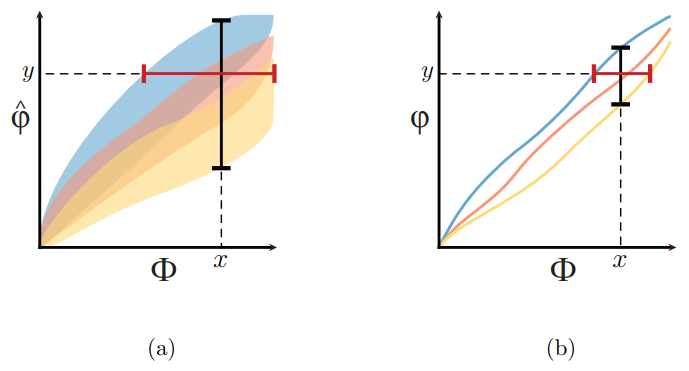
\includegraphics[scale = 0.4]{reshef_2015_fig1.png}
		\caption{
			\label{reshef_2015_f1}
			Una ilustraci\'on esquem\'atica de intervalos confiables e interpretables. En ambas partes de la figura, $\mathcal{Q}$ consiste en relaciones ruidosas de tres tipos diferentes representados en tres colores distintos. (a) La relaci\'on entre un estad\'istico $\hat{\varphi}$ y $\Phi$ en $\mathcal{Q}$ en un tama\~no de muestra finito. Los l\'imites inferior y superior de cada regi\'on sombreada indican los percentiles $(\alpha / 2) \cdot 100 \%$ y $(1 - \alpha / 2) \cdot 100 \%$ de la distribuci\'on de muestreo de $\hat{\varphi}$ para cada tipo de relaci\'on en varios valores de $\Phi$. El intervalo vertical (en negro) es el intervalo confiable $R_\alpha^{\hat{\varphi}}(x)$, y el intervalo horizontal (en rojo) es el intervalo interpretable $I_\alpha^{\hat{\varphi}}(y)$. (b) En el l\'imite de muestra grande, reemplazamos $\hat{\varphi}$ por una cantidad poblacional $\varphi$. El intervalo vertical (en negro) es el intervalo confiable $R^{\varphi}(x)$, y el intervalo horizontal (en rojo) es el intervalo interpretable $I^{\varphi}(y)$.}
	\end{figure}

	\section{Definiendo Equitabilidad}

	La proposici\'on \ref{interpretabilidad} implica que si los intervalos de interpretabilidad de $\hat{\varphi}$ con respecto a $\Phi$ son pequen\~os, entonces $\hat{\varphi}$ dar\'a buenos intervalos de estimac\'on de $\Phi$. Hay variadas formas de resumir si los intervalos de interpretabilidad son peque\~nos; nos enfocaremos en dos formas simples de hacerlo.
	
	\begin{defn}[$\alpha$-fiabilidad y $\alpha$-interpretabilidad]
		La \textit{$\alpha$-fiabilidad (resp. $\alpha$-interpretabilidad) en caso peor} de $\hat{\varphi}$ es $1/d$ si es $1/d$-fiable (resp. interpretable) para todo $x$ (resp. $y$) $\in [0,1]$. Se dice que $\hat{\varphi}$ es \textit{$1/d$-fiable (resp. $\alpha$-interpretable) en caso peor} con probabilidad (resp. confianza) $1-\alpha$.

		La \textit{$\alpha$-fiabilidad (resp. $\alpha$-interpretabilidad) en caso promedio} de $\hat{\varphi}$ es $1/d$ si su fiabilidad (resp. interpretabilidad), promediada sobre todo $x$ (resp. $y$) $\in [0,1]$, es al menos $1/d$. Se dice que $\hat{\varphi}$ es \textit{$1/d$-fiable (resp. $\alpha$-interpretable) en caso promedio} con probabilidad (resp. confianza) $1-\alpha$
	\end{defn}

	Con este vocaculario, podemos definir equitabilidad.

	\begin{defn}
		La \textit{Equitabilidad en caso promedio/peor} es simplemente \textit{interpretabilidad en caso promedio/peor} con respecto a un $\Phi$ que refeleje la fuerza de la relaci\'on. 
	\end{defn}

	\begin{rem}
		Notemos que Equitabilidad es un caso en particular de interpretabilidad donde $\Phi$ cumple un rol en especifico. Es posible definir un $\Phi$ que mida otras propiedades y resalte otro tipo de relaci\'ones. En este trabajo usaremos $R^2$ para medir fuerza entre relaciones, ahondaremos m\'as en esto en la siguiente secci\'on.
	\end{rem}

	Las definiciones correspondientes de interpretabilidad/fiablidad en caso promedio/peor son posibles para $\varphi$ in el caso de l\'imite para muestras grandes. En este caso, es posible que todos los intervalos de interpretabilidad de $\varphi$ con respecto a $\Phi$ tengan taman\~o 0, esto es, que el valor de $\varphi(Z)$ determina \'unicamente el valor de $\Phi(Z)$. En este caso, la interpretabilidad/fiablidad en caso promedio/peor de $\varphi$ es $\infty$, y se dice que $\varphi$ es perfectamente interpretable/fiable, o perfectamente equitativo dependiendo del contexto.

	Antes de seguir con la siguiente secci\'on, con el objetivo de construir intuici\'on, vamos a presentar dos ejemplos de estadi\'isticos que son perfectamente interpretables en el caso 
	l\'imite para muestras grandes. Primero, la Informaci\'on M\'utua \cite{inftheo2006}\cite{inftheo2008} es perfectamente interpretable con respecto a la correlaci\'on $\rho^2$ en el conjunto $\mathcal{Q}$ de vectores normales bivariados. Esto es dado que para normales bivariadas tenemos que $1-2^{-2I} = \rho^2$ \cite{infcorr}. Adicionalmente, el Teorema 6 de \cite{Szekely2009} muestra que para normales bivariadas, la correlaci\'on por distancia es tambi\'en es una funci\'on completamente determinada por $\rho^2$. Por lo tanto, la correlaci\'on por distancia tambi\'en es perfectamente interpretable y perfectamentef fiable con respecto a $\phi^2$ en el conjunto normales bivariadas $\mathcal{Z}$.

	La interpretabilidad perfecta con respecto a $\rho^2$ en bivariadas normales exhibida en ambos ejemplos es de hecho equivalente a una de las ''propiedades fundamentales'' introducidas por R\'enyi en su m\'etodo para evaluar las propiedades ideales de medidas de dependencia \cite{renyi1959}. Esto contiene un compromiso: Por un lado garantiza interpretabilidad perfecta, pero por el otro, solo aplica en un conjunto de relaciones relativamente pequen\~o. Uno de los objetivo de la Equitabilidad es relajar el requermiento de ''perfecci\'on'' a cambio de la habilidad de aplicar a un conjunto de relaciones m\'as amplio, por ejemplo, un conjuntod e funcionales ruidosos. Por tanto, es posible ver la equitabilidad como una generalizaci\'on de los requermiento de R\'enyi que nos permite hacer un intercambio entre la precisi\'on con la que nuestro estad\'istico nos informa sobre $\Phi$ y el conjunto $\mathcal{Q}$ sobre el cu\'al act\'ua.
	
	\section[interpretabilidad sobre r2]{Interpretabilidad sobre $R^2$}

	Durante este cap\'itulo hemos mencionado el concepto de relaciones funcionales ruidosas y de $R^2$, ahora los definimos de forma formal. Comenzemos primero con $R^2$
	\begin{defn}[$R^2$]
		Sea $y=[y_1,\dots,y_n]\in\R^n$ un vector de muestras de una variable aleatoria y sea $f:\R\to\R$ una funci\'on que modela la variable aleatoria, definamos $f_i:=f(y_i)$. El coeficiente de determinaci\'on o $R^2$ se define como:

		$$
		R^2 = 1 - \frac{\sum_i(y_i-f_i)^2}{\sum_i(y_i-\bar{y})^2},
		$$

		donde $\sum_i(y_i-f_i)^2$ corresponde a la suma del cuadrado de los residuales, $\sum_i(y_i-\bar{y})^2$ es la suma total de cuadrados (proporcional a la varianza), e $\hat{y}$ es el promedio de la muestra.
	\end{defn}

	En palabras simples, $R^2$ es la proporci\'on de variaci\'on en la variable dependiente que puede ser explicado por la variable independiente. Notemos que al momento de hacer el an\'alisis de equitabilidad, tenemos total claridad de cual es nuestra funci\'on $f$, dado que nosotros definimos la relaci\'on. Veamos ahora la siguiente definici\'on.	
		
	\begin{defn}[Relaci\'on Funcional Ruidosa]
		Una variable aleatoria distribuida sobre $\R^2$ es llamada una \textit{relaci\'on funcional ruidosa} si, y solo si, puede ser escrita en la forma $(X+\epsilon, f(X)+\epsilon\prime)$, donde $f:[0,1]\to\R$, $X$ es una variable aleatoria distribuida sobre $[0,1]$, y $\epsilon$ y $\epsilon\prime$ son (posiblemente nulas) distribuciones aleatorias. Denotamos el conjunto de todas las relaciones funcionales ruidosas como $\mathcal{F}$
		\label{ruido_func}
	\end{defn}

	Ya con esto, tenemos todo lo que necesitamos para definir la equitabilidad que usaremos para los an\'alisis de la siguiente secci\'on: Equitabilidad sobre $R^2$

	\begin{defn}[Equitabilidad en relaciones funcionales sobre $R^2$]
		Sea $\mathcal{Q}\in\mathcal{F}$ un conjunto de relaciones funcionales ruidosas. Una medida de dependencia es $1/d$-equitativa en $\mathcal{Q}$ con respecto a $R^2$ si es $1/d$-interpretable sobre $R^2$ en $\mathcal{Q}$ 
	\end{defn}

	Es necesario destacar que esta definici\'on aun depende del conjunto $\mathcal{Q}$ en cuesti\'on. El m\'etodo generalmente utilizado en la literatura ha sido fijar un conjunto $F$ de funciones tales que sean lo suficientemente grandes como para ser representativo de las relaciones encontradas en datos reales, pero que por otro lado sean lo suficientemente pequen\~nos tal que permitan an\'alsis emp\'irico. Discutiremos el $F$ a ultilziar en la siguiente secci\'on, donde realizaremos un ana\'alisis de equitabilidad sobre los estad\'isticos definidos en este trabajo.

	Tan importante como la elecc\'ion de funciones a incluir en $F$, es la elecci\'on de distribuciones marginales y el ruido, los cuales fueron no son especificados en la definici\'on \ref{ruido_func}. Varias posibilidades han sido propuestas por Reshef et al. \cite{Reshef2015a}, pero la m\'as utilizada en la literatura, y la que usaremos en la siguiente secci\'on, continua siendo la m\'as simple con $X\sim Unif$, $\epsilon\prime\sim\mathcal{N}(0,\sigma^2)$ con $\sigma$ variable y $\epsilon\equiv0$. 

	
	\section[equitabilidadmice]{Equitabilidad de las medidas}

	\todo{esta secci\'on está extraida de la secci\'on en el paper, la idea es hacer un an\'alisis similar para todas medidas propuestas
	}
	
	Como se mencion\'o previamente, una de las principales motivaciones para la introducci\'on de $MIC$ fue la equidad, es decir, hasta qu\'e punto una medida de dependencia captura \'utilmente alguna noci\'on de la fuerza de una relaci\'on en un conjunto de relaciones est\'andar. En esto contexto en Reshef et al. (2016) \cite{Reshef2016} se realiz\~o un an\'alisis emp\'irico de la equidad de $MIC_e$ con respecto a R2 y su desempe\~no fue comparado con la correlaci\'on de distancia (Sz\'ekely et al., (2007)\cite{Szekely2007}; Sz\'ekely and Rizzo, (2009)\cite{Szekely2009}), la estimaci\'on de la informaci\'on mutua (Kraskov et al., 2004) y la estimaci\'on de la correlaci\'on m\'axima (Breiman and Friedman, 1985).

	Se comenz\'o evaluando la equidad en el conjunto de relaciones $Q$ definido anteriormente, un conjunto que ha sido analizado en otros trabajos previos (Reshef et al., 2011, 2015a; Kinney and Atwal, 2014). Los resultados, mostrados en la Figura \ref{reshef_2016_f3}, confirman la superior equidad del estimador $MIC_e$ en este conjunto de relaciones.

	Para evaluar la equidad de manera m\'as objetiva sin depender de un conjunto de funciones curado manualmente, se analizaron 160 funciones aleatorias extra\'idas de una distribuci\'on de proceso Gaussiano con un kernel de funci\'on radial con una de ocho posibles anchuras en el conjunto $\{0.01, 0.025, 0.05, 0.1, 0.2, 0.25, 0.5, 1\}$ para representar una variedad de complejidades de relaciones posibles. Los resultados, mostrados en la Figura \ref{reshef_2016_f4}, muestran que $MIC_e$ supera a los m\'etodos existentes en t\'erminos de equidad con respecto a $R^2$ en estas funciones tambi\'en. Tambi\'en se examin\'o el efecto de las relaciones at\'ipicas en los resultados al muestrear repetidamente subconjuntos aleatorios de 20 funciones de este gran conjunto de relaciones y medir la equidad de cada m\'etodo en promedio sobre los subconjuntos; los resultados fueron similares.

	Una caracter\'istica del desempe\~no de $MIC_e$ en estas relaciones elegidas al azar, como se muestra en la Figura \ref{reshef_2016_f4}, es que parece ser m\'inimamente sensible a la anchura del proceso Gaussiano del cual se extrae una relaci\'on dada. Esto contrasta, por ejemplo, con la estimaci\'on de la informaci\'on mutua, que muestra una sensibilidad pronunciada a este par\'ametro que le impide ser altamente equitativa cuando hay relaciones con diferentes anchuras en el mismo conjunto de datos.

	\begin{figure}[H] 
		\centering
		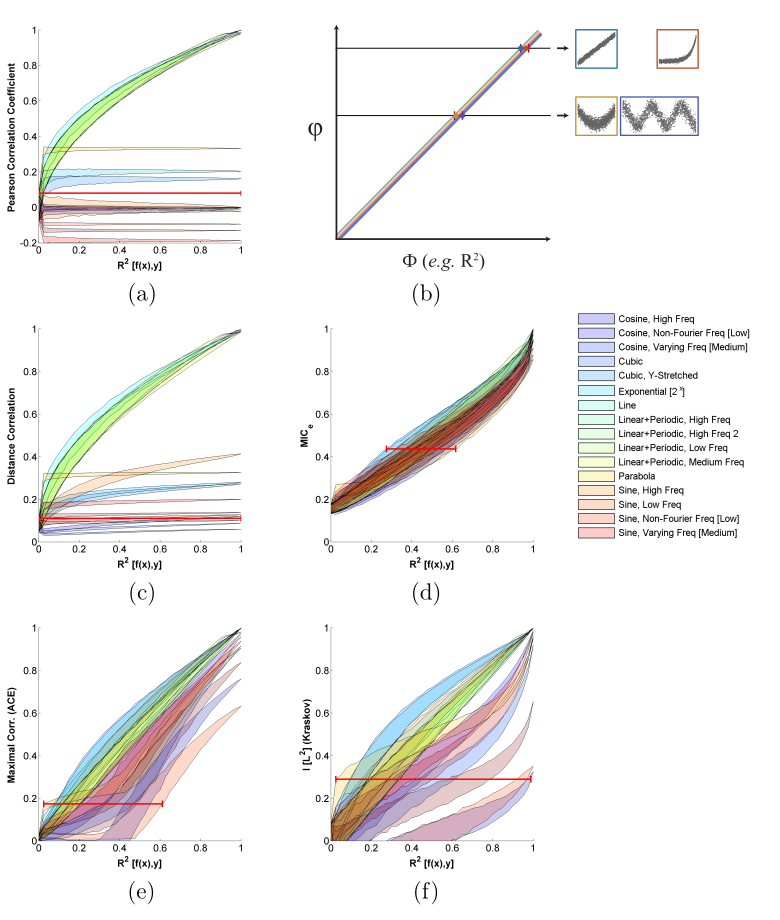
\includegraphics[scale = 0.4]{reshef_2016_fig3.png}
		\caption{Equitabilidad con respecto a $R^2$ en un conjunto de relaciones funcionales ruidosas de $(a)$ el coeficiente de correlaci\~on de Pearson, $(b)$ una medida hipot\~etica de dependencia $\varphi$ con equitabilidad perfecta, $(c)$ la correlaci\~on de distancia, $(d)$ $\mathrm{MIC}_e$, $(e)$ estimaci\~on de correlaci\~on m\~axima y $(f)$ estimaci\~on de informaci\~on mutua. Para cada relaci\~on, una regi\~on sombreada denota los valores estimados en el percentil 5 y 95 de la distribuci\~on muestral de la estad\~istica en cuesti\~on en esa relaci\~on en cada valor de $R^2$. El gr\~afico resultante muestra qu\~e valores de $R^2$ corresponden a un valor dado de cada estad\~istica. El intervalo rojo en cada gr\~afico indica el rango m\~as amplio de valores de $R^2$ que corresponden a un valor de la estad\~istica; cuanto m\~as estrecho sea el intervalo rojo, mayor ser\~a la equitabilidad. Un intervalo rojo con ancho 0, como en $(b)$, significa que la estad\~istica refleja solo $R^2$ sin depender del tipo de relaci\~on, como se demuestra en los pares de miniaturas de relaciones de diferentes tipos con valores id\~enticos de $R^2$.}
		\label{reshef_2016_f3}
	\end{figure}

	\begin{figure}[H] 
		\centering
		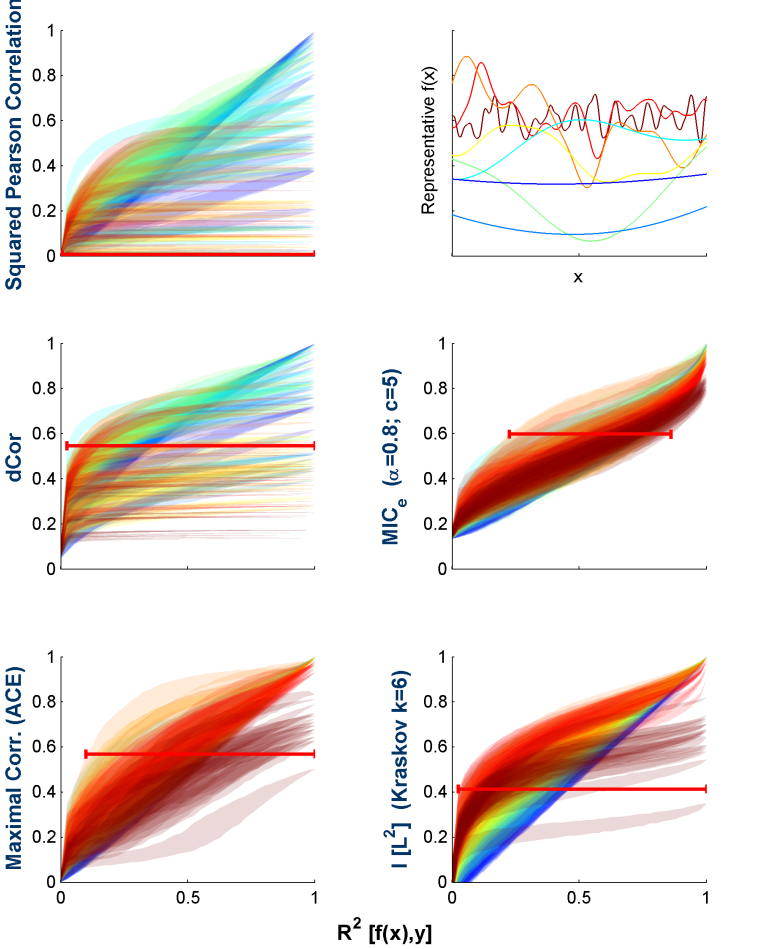
\includegraphics[scale = 0.4]{reshef_2016_fig4.png}
		\caption{Equitabilidad de los m\~etodos examinados en funciones extra\~idas al azar de una distribuci\~on de proceso gaussiano. Cada m\~etodo se eval\~ua como se muestra en la Figura \ref{reshef_2016_f3}, con un intervalo rojo que indica el rango m\~as amplio de valores de $R^2$ correspondiente a cualquier valor de la estad\~istica; cuanto m\~as estrecho sea el intervalo rojo, mayor ser\~a la equitabilidad. Cada regi\~on sombreada corresponde a una relaci\~on, y las regiones est\~an coloreadas seg\~un el ancho de banda del proceso gaussiano del que se muestrearon. Las relaciones de muestra para cada ancho de banda se muestran en la esquina superior derecha con colores correspondientes.}
		\label{reshef_2016_f4}
	\end{figure}